\chapter{Google}
Google interview questions
\newline

\section{Odd Even Jump} %%%%%%%%%%%%%%%%%%%%%%%%%%%%%%
\label{sec:odd-even-jump}


\subsubsection{描述}
You are given an integer array A.  From some starting index, you can make a series of jumps.  The (1st, 3rd, 5th, ...) jumps in the series are called odd numbered jumps, and the (2nd, 4th, 6th, ...) jumps in the series are called even numbered jumps.

You may from index i jump forward to index j (with i < j) in the following way:

During odd numbered jumps (ie. jumps 1, 3, 5, ...), you jump to the index j such that A[i] <= A[j] and A[j] is the smallest possible value.  If there are multiple such indexes j, you can only jump to the smallest such index j.
During even numbered jumps (ie. jumps 2, 4, 6, ...), you jump to the index j such that A[i] >= A[j] and A[j] is the largest possible value.  If there are multiple such indexes j, you can only jump to the smallest such index j.
(It may be the case that for some index i, there are no legal jumps.)
A starting index is good if, starting from that index, you can reach the end of the array (index A.length - 1) by jumping some number of times (possibly 0 or more than once.)

Return the number of good starting indexes.

Example 1:
\begin{Code}
Input: [10,13,12,14,15]
Output: 2
Explanation:
From starting index i = 0, we can jump to i = 2 (since A[2] is the smallest among A[1], A[2], A[3], A[4] that is greater or equal to A[0]), then we can't jump any more.
From starting index i = 1 and i = 2, we can jump to i = 3, then we can't jump any more.
From starting index i = 3, we can jump to i = 4, so we've reached the end.
From starting index i = 4, we've reached the end already.
In total, there are 2 different starting indexes (i = 3, i = 4) where we can reach the end with some number of jumps.
\end{Code}

Example 2:
\begin{Code}
Input: [2,3,1,1,4]
Output: 3
Explanation:
From starting index i = 0, we make jumps to i = 1, i = 2, i = 3:

During our 1st jump (odd numbered), we first jump to i = 1 because A[1] is the smallest value in (A[1], A[2], A[3], A[4]) that is greater than or equal to A[0].

During our 2nd jump (even numbered), we jump from i = 1 to i = 2 because A[2] is the largest value in (A[2], A[3], A[4]) that is less than or equal to A[1].  A[3] is also the largest value, but 2 is a smaller index, so we can only jump to i = 2 and not i = 3.

During our 3rd jump (odd numbered), we jump from i = 2 to i = 3 because A[3] is the smallest value in (A[3], A[4]) that is greater than or equal to A[2].

We can't jump from i = 3 to i = 4, so the starting index i = 0 is not good.

In a similar manner, we can deduce that:
From starting index i = 1, we jump to i = 4, so we reach the end.
From starting index i = 2, we jump to i = 3, and then we can't jump anymore.
From starting index i = 3, we jump to i = 4, so we reach the end.
From starting index i = 4, we are already at the end.
In total, there are 3 different starting indexes (i = 1, i = 3, i = 4) where we can reach the end with some number of jumps.
\end{Code}

Example 3:
\begin{Code}
Input: [5,1,3,4,2]
Output: 3
Explanation:
We can reach the end from starting indexes 1, 2, and 4.
\end{Code}


\subsubsection{動規 - Monotonic Stack}
\begin{Code}
// 思路: 先求得單和雙數往後跳的目的地,再用動規,得知由某點能否跳往目的地
// 時間複雜度O(nlogn),空間複雜度O(n)
class Solution {
public:
    int oddEvenJumps(vector<int>& A) {
        vector<pair<int, int>> cache; cache.reserve(A.size());
        for (int i = 0; i < A.size(); i++)
            cache.emplace_back(A[i], i);
        // 找尋增大順序的下標
        sort(cache.begin(), cache.end()
             , [&](const auto& left, const auto& right)
             {
                 if (left.first == right.first)
                     return left.second < right.second;
                 else
                     return left.first < right.first;
             });
        vector<int> sortedIndex;
        sortedIndex.reserve(cache.size());
        for_each(cache.begin(), cache.end()
                , [&](const auto& ele) { sortedIndex.push_back(ele.second); } );
        // 求得單數跳躍的下標
        vector<int> oddNext = GetNext(sortedIndex);

        // 找尋減少順序的下標
        sort(cache.begin(), cache.end()
             , [&](const auto& left, const auto& right)
             {
                 if (left.first == right.first)
                     return left.second < right.second;
                 else
                     return left.first > right.first;
             });
        sortedIndex.clear();
        sortedIndex.reserve(cache.size());
        for_each(cache.begin(), cache.end()
                , [&](const auto& ele) { sortedIndex.push_back(ele.second); } );
        // 求得雙數跳躍的下標
        vector<int> evenNext = GetNext(sortedIndex);

        // 設 odd[i]: 單數跳躍時可以由 i 到 N
        vector<bool> odd(A.size(), false);
        // 設 even[i]: 雙數跳躍時可以由 i 到 N
        vector<bool> even(A.size(), false);
        odd.back() = even.back() = true;

        // odd 的總數便是答案
        for (int i = A.size() - 1; i >= 0; i--)
        {
            if (oddNext[i] != -1)
                odd[i] = even[oddNext[i]];
            if (evenNext[i] != -1)
                even[i] = odd[evenNext[i]];
        }

        int result = 0;
        for (const auto& o : odd)
            if (o) result++;

        return result;
    }
private:
    vector<int> GetNext(const vector<int>& inputIndex)
    {
        // 使用了 Monotonic Stack
        stack<int> cache;
        vector<int> result(inputIndex.size(), -1); // -1 代表沒法再往後跳躍

        for (const auto& index : inputIndex)
        {
            while (!cache.empty() && cache.top() < index)
            {
                result[cache.top()] = index;
                cache.pop();
            }
            cache.push(index);
        }

        return result;
    }
};
\end{Code}

\subsubsection{動規 - Map}
\begin{Code}
// 思路: 利用 BST 由尾至頭歷遍,找出每一個對應的跳躍目的地
// 時間複雜度O(nlogn),空間複雜度O(n)
class Solution {
public:
    int oddEvenJumps(vector<int>& A) {
        int N = A.size();
        // 設 odd[i]: 單數跳躍時可以由 i 到 N
        vector<bool> odd(A.size(), false);
        // 設 even[i]: 雙數跳躍時可以由 i 到 N
        vector<bool> even(A.size(), false);
        odd.back() = even.back() = true;

        map<int, int> cache; // key: A[i] value: i
        cache.emplace(A[N-1], N-1);

        for (int i = N - 2; i >= 0; i--)
        {
            auto it = cache.find(A[i]);
            if (it != cache.end())
            {
                odd[i] = even[it->second];
                even[i] = odd[it->second];
            }
            else
            {
                auto bigger = GetBigger(cache, A[i]);
                auto smaller = GetSmaller(cache, A[i]);

                if (bigger != cache.end())
                    odd[i] = even[bigger->second];
                if (smaller != cache.end())
                    even[i] = odd[smaller->second];
            }
            cache[A[i]] = i;
        }

        // odd 的總數便是答案
        int result = 0;
        for (const auto& o : odd)
            if (o) result++;

        return result;
    }
private:
    template <class MyMap, class T>
        typename MyMap::iterator GetBigger(MyMap& cache, T val)
    {
        auto bigger = cache.lower_bound(val);
        if (bigger == cache.end())
            return bigger;
        else
            return bigger;
    }
    template <class MyMap, class T>
        typename MyMap::iterator GetSmaller(MyMap& cache, T val)
    {
        auto smaller = cache.lower_bound(val);
        if (smaller == cache.begin())
            return cache.end();
        else
            return prev(smaller);
    }
};
\end{Code}

\subsubsection{動規 - Multimap}
\begin{Code}
// 思路: 利用 BST 由尾至頭歷遍,找出每一個對應的跳躍目的地
// 時間複雜度O(nlogn),空間複雜度O(n)
class Solution {
public:
    int oddEvenJumps(vector<int>& A) {
        int N = A.size();
        // 設 odd[i]: 單數跳躍時可以由 i 到 N
        vector<bool> odd(A.size(), false);
        // 設 even[i]: 雙數跳躍時可以由 i 到 N
        vector<bool> even(A.size(), false);
        odd.back() = even.back() = true;

        multimap<int, int> cache; // key: A[i] value: i
        cache.emplace(A[N-1], N-1);

        for (int i = N - 2; i >= 0; i--)
        {
            auto it = cache.find(A[i]);
            if (it != cache.end())
            {
                // 找尋同值最細下標
                it = GetSmallestIndex(cache, it);
                odd[i] = even[it->second];
                even[i] = odd[it->second];
            }
            else
            {
                auto bigger = GetBigger(cache, A[i]);
                auto smaller = GetSmaller(cache, A[i]);

                if (smaller != cache.end())
                    even[i] = odd[smaller->second];
                if (bigger != cache.end())
                    odd[i] = even[bigger->second];
            }
            cache.emplace(A[i], i);
        }

        // odd 的總數便是答案
        int result = 0;
        for (const auto& o : odd)
            if (o) result++;

        return result;
    }
private:
    template <class MyMap, class T>
        typename MyMap::iterator GetBigger(MyMap& cache, T val)
    {
        auto bigger = cache.lower_bound(val);
        if (bigger == cache.end())
            return bigger;
        else
            return GetSmallestIndex(cache, bigger); // 找尋同值最細下標
    }
    template <class MyMap, class T>
        typename MyMap::iterator GetSmaller(MyMap& cache, T val)
    {
        auto smaller = cache.lower_bound(val);
        if (smaller == cache.begin())
            return cache.end();
        else
            return GetSmallestIndex(cache, prev(smaller)); // 找尋同值最細下標
    }
    template <class MyMap, class MapIT>
        MapIT GetSmallestIndex(MyMap& cache, MapIT target)
    {
        auto range = cache.equal_range(target->first);
            // 找尋同值最細下標
            int minIndex = INT_MAX;
            for (auto j = range.first; j != range.second; j++)
            {
                if (minIndex > j->second)
                {
                    target = j;
                    minIndex = j->second;
                }
            }

        return target;
    }
};
\end{Code}

\section{Course Schedule II} %%%%%%%%%%%%%%%%%%%%%%%%%%%%%%
\label{sec:course-schedule-ii}


\subsubsection{描述}
There are a total of n courses you have to take, labeled from 0 to n-1.

Some courses may have prerequisites, for example to take course 0 you have to first take course 1, which is expressed as a pair: [0,1]

Given the total number of courses and a list of prerequisite pairs, return the ordering of courses you should take to finish all courses.

There may be multiple correct orders, you just need to return one of them. If it is impossible to finish all courses, return an empty array.

Example 1:
\begin{Code}
Input: 2, [[1,0]]
Output: [0,1]
Explanation: There are a total of 2 courses to take.
             To take course 1 you should have finished
             course 0. So the correct course order is [0,1] .
\end{Code}

Example 2:
\begin{Code}
Input: 4, [[1,0],[2,0],[3,1],[3,2]]
Output: [0,1,2,3] or [0,2,1,3]
Explanation: There are a total of 4 courses to take.
             To take course 3 you should have finished both courses 1 and 2.
             Both courses 1 and 2 should be taken after you finished course 0.
             So one correct course order is [0,1,2,3].
             Another correct ordering is [0,2,1,3] .
\end{Code}

Note:
\begindot
\item The input prerequisites is a graph represented by a list of edges, not adjacency matrices. Read more about how a graph is represented.
\item You may assume that there are no duplicate edges in the input prerequisites.
\myenddot

\subsubsection{DFS - Topological Sort}
\begin{Code}
// 時間複雜度O(n),空間複雜度O(n)
class Solution {
public:
    vector<int> findOrder(int numCourses, vector<vector<int>>& prerequisites) {
        vector<int> result; result.reserve(numCourses);

        // Topological Sort
        // 先造出 dependency graph
        // 也記低有什麼 course 出現過
        unordered_map<int, list<int>> dGraph;
        unordered_set<int> seenCourse;
        for (const auto& p : prerequisites)
        {
            dGraph[p[0]].push_back(p[1]);
            seenCourse.insert(p[0]);
            seenCourse.insert(p[1]);
        }

        // 先補上在 graph 中沒有出現的 course
        for (int i = 0; i < numCourses; i++)
            if (seenCourse.count(i) == 0) result.push_back(i);

        // 利用 DFS 造出答案
        unordered_map<int, bool> visited;

        for (const auto& [k, v] : dGraph)
        {
            if (!DFS(dGraph, k, result, visited)) return vector<int>();
        }

        return result;
    }
private:
    bool DFS(const unordered_map<int, list<int>>& dGraph, int k
             , vector<int>& result, unordered_map<int, bool>& visited)
    {
        if (visited.find(k) != visited.end()) return visited[k];

        visited[k] = false;

        auto it = dGraph.find(k);
        if (it != dGraph.end())
        {
            for (const auto& nei : it->second)
            {
                if (!DFS(dGraph, nei, result, visited)) return false;
            }
        }

        visited[k] = true;
        result.push_back(k);

        return true;
    }
};
\end{Code}

\section{Longest Increasing Path in a Matrix} %%%%%%%%%%%%%%%%%%%%%%%%%%%%%%
\label{sec:longest-increasing-path-in-a-matrix}


\subsubsection{描述}
Given an integer matrix, find the length of the longest increasing path.

From each cell, you can either move to four directions: left, right, up or down. You may NOT move diagonally or move outside of the boundary (i.e. wrap-around is not allowed).

Example 1:
\begin{Code}
Input: nums =
[
  [9,9,4],
  [6,6,8],
  [2,1,1]
]
Output: 4
Explanation: The longest increasing path is [1, 2, 6, 9].
\end{Code}

Example 2:
\begin{Code}
Input: nums =
[
  [3,4,5],
  [3,2,6],
  [2,2,1]
]
Output: 4
Explanation: The longest increasing path is [3, 4, 5, 6]. Moving diagonally is not allowed.
\end{Code}


\subsubsection{備忘錄法}
\begin{Code}
// 時間複雜度O(m*n),空間複雜度O(m*n)
class Solution {
public:
    int longestIncreasingPath(vector<vector<int>>& matrix) {
        m_M = matrix.size();
        if (m_M == 0) return 0;
        m_N = matrix[0].size();
        if (m_N == 0) return 0;

        vector<vector<bool>> visited(m_M, vector<bool>(m_N, false));
        // 設 cache[i][j] 為 i,j 的最長答案
        // 這個答案是由 0 開始總加的,所以 DFS 也要由 0 開始總加
        vector<vector<int>> cache(m_M, vector<int>(m_N, -1));
        int maxLen = INT_MIN;
        for (int i = 0; i < m_M; i++)
        {
            for (int j = 0; j < m_N; j++)
            {
                maxLen = max(maxLen, DFS(i, j, matrix, cache, visited));
            }
        }


        return maxLen;
    }
private:
    const vector<pair<int, int>> directions{{1,0}, {0,1}, {-1,0}, {0,-1}};
    int DFS(int i, int j, const vector<vector<int>>& matrix
            , vector<vector<int>>& cache, vector<vector<bool>>& visited)
    {
        if (cache[i][j] != -1) return cache[i][j];

        visited[i][j] = true;
        int maxLen = 0;
        for (int d = 0; d < 4; d++)
        {
            int newI = i + directions[d].first;
            int newJ = j + directions[d].second;
            if (newI >= 0 && newI < m_M && newJ >= 0 && newJ < m_N
                && !visited[newI][newJ]
                && matrix[i][j] > matrix[newI][newJ])// 由大至細地找尋答案 (由細至大也可以)
                maxLen = max(maxLen, DFS(newI, newJ, matrix, cache, visited));
        }
        visited[i][j] = false;

        return cache[i][j] = maxLen + 1; // 注意: 由細至大保存中途答案
    }
private:
    int m_M;
    int m_N;
};
\end{Code}

\section{Count Complete Tree Nodes} %%%%%%%%%%%%%%%%%%%%%%%%%%%%%%
\label{sec:count-complete-tree-nodes}


\subsubsection{描述}
Given a complete binary tree, count the number of nodes.

Note:

Definition of a complete binary tree from Wikipedia:
In a complete binary tree every level, except possibly the last, is completely filled, and all nodes in the last level are as far left as possible. It can have between 1 and 2h nodes inclusive at the last level h.

Example:
\begin{Code}
Input:
    1
   / \
  2   3
 / \  /
4  5 6

Output: 6
\end{Code}


\subsubsection{暴力}
\begin{Code}
// 時間複雜度O(n),空間複雜度O(n)
class Solution {
public:
    int countNodes(TreeNode* root) {
        if (root == nullptr) return 0;

        return 1 + countNodes(root->left) + countNodes(root->right);
    }
};
\end{Code}

\subsubsection{Binary Search}
\begin{Code}
// 時間複雜度O(d^2),空間複雜度O(n)
class Solution {
public:
    int countNodes(TreeNode* root) {
        // 若果樹沒有元素
        if (root == nullptr) return 0;

        int d = ComputeDepth(root);
        // 若果樹只有一個元素
        if (d == 0) return 1;

        // left: 為最低層的最左的 node index
        // right: 為最低層的最右的 node index
        int left = 1; int right = pow(2, d) - 1;
        while (left <= right)
        {
            int pivot = (left + right) / 2;
            if (IsExist(pivot, d, root))
                left = pivot + 1;
            else
                right = pivot - 1;
        }

        return pow(2, d) - 1 + left;
    }
private:
    int ComputeDepth(TreeNode *root)
    {
        int d = 0;
        while (root->left)
        {
            root = root->left;
            d++;
        }
        return d;
    }
    bool IsExist(int idx, int d, TreeNode* node)
    {
        int left = 0; int right = pow(2, d) - 1;
        for (int i = 0; i < d; i++)
        {
            int pivot = (left + right) / 2;
            if (idx <= pivot)
            {
                node = node->left;
                right = pivot;
            }
            else
            {
                node = node->right;
                left = ++pivot;
            }
        }
        return node != nullptr;
    }
};
\end{Code}

\section{Flip Equivalent Binary Trees} %%%%%%%%%%%%%%%%%%%%%%%%%%%%%%
\label{sec:flip-equivalent-binary-trees}


\subsubsection{描述}
For a binary tree T, we can define a flip operation as follows: choose any node, and swap the left and right child subtrees.

A binary tree X is flip equivalent to a binary tree Y if and only if we can make X equal to Y after some number of flip operations.

Write a function that determines whether two binary trees are flip equivalent.  The trees are given by root nodes root1 and root2.

Example 1:
\begin{Code}
Input:
       1                 1
      /  \              / \
     3    2            2   3
      \  / \          / \  /
      6 4   5        4  5 6
           / \         / \
          8   7       7   8

Input: root1 = [1,2,3,4,5,6,null,null,null,7,8], root2 = [1,3,2,null,6,4,5,null,null,null,null,8,7]
Output: true
Explanation: We flipped at nodes with values 1, 3, and 5.
\end{Code}

Note:
\begindot
\item Each tree will have at most 100 nodes.
\item Each value in each tree will be a unique integer in the range [0, 99]
\myenddot


\subsubsection{遞歸}
\begin{Code}
// 時間複雜度O(min(N1, N2)),空間複雜度O(min(H1, H2))
class Solution {
public:
    bool flipEquiv(TreeNode* root1, TreeNode* root2) {
        if (root1 == nullptr) return root2 == nullptr;
        if (root2 == nullptr) return root1 == nullptr;

        return root1->val == root2->val
            && (flipEquiv(root1->right, root2->left) && flipEquiv(root1->left, root2->right)
                || flipEquiv(root1->right, root2->right) && flipEquiv(root1->left, root2->left));
    }
};
\end{Code}

\subsubsection{Canonical Traversal}
\begin{Code}
// 時間複雜度O(min(N1, N2)),空間複雜度O(min(H1, H2))
class Solution {
public:
    bool flipEquiv(TreeNode* root1, TreeNode* root2) {
        list<TreeNode*> vals1;
        list<TreeNode*> vals2;

        // 由細至大把二叉樹放到鏈表中
        DFS(root1, vals1);
        DFS(root2, vals2);

        // 當兩個表是一樣,回 true
        return vals1.size() == vals2.size()
            && equal(vals1.begin(), vals1.end(), vals2.begin()
                     , [](const auto& left, const auto& right)
                     {
                         if (left == nullptr && right == nullptr) return true;
                         else if (left == nullptr || right == nullptr) return false;
                         else return left->val == right->val;
                     });
    }
private:
    void DFS(TreeNode *root, list<TreeNode*>& vals)
    {
        if (root == nullptr) return;

        vals.push_back(root);

        int L = root->left == nullptr ? -1 : root->left->val;
        int R = root->right == nullptr ? -1 : root->right->val;

        if (L < R)
        {
            DFS(root->left, vals);
            DFS(root->right, vals);
        }
        else
        {
            DFS(root->right, vals);
            DFS(root->left, vals);
        }

        vals.push_back(nullptr);
    }
};
\end{Code}

\section{Diameter of Binary Tree} %%%%%%%%%%%%%%%%%%%%%%%%%%%%%%
\label{sec:diameter-of-binary-tree}


\subsubsection{描述}
Given a binary tree, you need to compute the length of the diameter of the tree. The diameter of a binary tree is the length of the longest path between any two nodes in a tree. This path may or may not pass through the root.

Example:
Given a binary tree
\begin{Code}
          1
         / \
        2   3
       / \     
      4   5    

Return 3, which is the length of the path [4,2,1,3] or [5,2,1,3].

Note: The length of path between two nodes is represented by the number of edges between them.
\end{Code}


\subsubsection{遞歸}
\begin{Code}
// 時間複雜度O(n),空間複雜度O(1)
class Solution {
public:
    int diameterOfBinaryTree(TreeNode* root) {
        m_result = 1;
        DFS(root);
        return m_result - 1;
    }
private:
    int DFS(TreeNode *root)
    {
        if (root == nullptr) return 0;

        int L = DFS(root->left);
        int R = DFS(root->right);

        m_result = max(m_result, L+R+1); // 由左至右總加起來
        return max(L, R) + 1; // 注意: 只取最長的子樹
    }
private:
    int m_result;
};
\end{Code}

\section{Evaluate Division} %%%%%%%%%%%%%%%%%%%%%%%%%%%%%%
\label{sec:evaluate-division}


\subsubsection{描述}
Equations are given in the format A / B = k, where A and B are variables represented as strings, and k is a real number (floating point number). Given some queries, return the answers. If the answer does not exist, return -1.0.

Example:
Given a / b = 2.0, b / c = 3.0.
queries are: a / c = ?, b / a = ?, a / e = ?, a / a = ?, x / x = ? .
return [6.0, 0.5, -1.0, 1.0, -1.0 ].

\begin{Code}
  The input is: vector<pair<string, string>> equations, vector<double>& values
  , vector<pair<string, string>> queries , where equations.size() == values.size()
  , and the values are positive. This represents the equations. Return vector<double>.
\end{Code}

According to the example above:

\begin{Code}
equations = [ ["a", "b"], ["b", "c"] ],
values = [2.0, 3.0],
queries = [ ["a", "c"], ["b", "a"], ["a", "e"], ["a", "a"], ["x", "x"] ]. 
\end{Code}

The input is always valid. You may assume that evaluating the queries will result in no division by zero and there is no contradiction.

\subsubsection{遞歸 - DFS}
\begin{Code}
// 時間複雜度O(n),空間複雜度O(n)
class Solution {
public:
    vector<double> calcEquation(vector<vector<string>>& equations
                                , vector<double>& values
                                , vector<vector<string>>& queries){
        // 造圖
        unordered_map<string,vector<pair<double,string>>> g;
        for (int i = 0; i < equations.size(); i++)
        {
            string& strA = equations[i][0];
            string& strB = equations[i][1];
            // 記錄 A / B
            g[strA].emplace_back(values[i], strB);
            // 記錄 B / A
            g[strB].emplace_back(1 / values[i], strA);
        }

        vector<double> result;
        for (int i = 0; i < queries.size(); i++)
        {
            const string& qStart = queries[i][0];
            const string& qEnd = queries[i][1];
            // 若整個除數關係沒有記錄
            if (g.find(qStart) == g.end() || g.find(qEnd) == g.end())
                result.push_back(-1.0);
            else
            {
                // 若有記錄
                set<string> visited;
                int ansLen = result.size();
                DFS(qStart, qEnd, 1, visited, result, g);
                if (result.size() == ansLen)
                    result.push_back(-1); // 若找不到答案
            }
        }
        return result ;
    }
private:
    void DFS(string start, string end, double cost
             , set<string>& visited
             , vector<double>& result
             , unordered_map<string,vector<pair<double,string>>>& g)
    {
        visited.insert(start);

        if (start == end)
        {
            result.push_back(cost);
            return;
        }

        for (const auto& [num, neigbor] : g[start])
        {
            if (visited.find(neigbor) != visited.end()) continue;

            int ansLen = result.size();
            DFS(neigbor, end, cost * num, visited, result, g);
            if (ansLen != result.size()) return; // 已找到答案,剪枝
        }
    }
};
\end{Code}

\section{Cracking the Safe} %%%%%%%%%%%%%%%%%%%%%%%%%%%%%%
\label{sec:cracking-the-safe}


\subsubsection{描述}
There is a box protected by a password. The password is a sequence of n digits where each digit can be one of the first k digits 0, 1, ..., k-1.

While entering a password, the last n digits entered will automatically be matched against the correct password.

For example, assuming the correct password is "345", if you type "012345", the box will open because the correct password matches the suffix of the entered password.

Return any password of minimum length that is guaranteed to open the box at some point of entering it.

Example 1:
\begin{Code}
Input: n = 1, k = 2
Output: "01"
Note: "10" will be accepted too.
\end{Code}

Example 2:
\begin{Code}
Input: n = 2, k = 2
Output: "00110"
Note: "01100", "10011", "11001" will be accepted too.
\end{Code}

Note:
\begindot
\item n will be in the range (1, 4).
\item k will be in the range (1, 10).
\item pow(k, n) will be at most 4096.
\myenddot

\subsubsection{遞歸 - DFS - Hierholzer's Algorithm}
\begin{Code}
// 時間複雜度O(n * k^n),空間複雜度O(n * k^n)
// 利用 Hierholzer's Algorithm 歷遍所有 edges 並記錄所有的 nodes
// Hierholzer's Algorithm 用來找尋 Eulerian Path
class Solution {
public:
    string crackSafe(int n, int k) {
        if (n == 1 && k == 1) return "0";
        // seen 用來存放見過的 node
        unordered_set<string> seen;
        string result;

        // 準備開始點
        string start; start.append(n-1, '0');

        DFS(start, k, seen, result);
        result += start;

        return result;
    }
private:
    void DFS(const string& node, int k, unordered_set<string>& seen, string& result)
    {
        // 這是 post order travel 的做法
        for (int x = 0; x < k; x++)
        {
            // nei 是下一個歷遍的 node + edge
            // x 為 edge, 0, 1, 2 ... k-1
            string nei = node + to_string(x);
            if (seen.find(nei) == seen.end())
            {
                seen.insert(nei);
                // nei.substr(1) 可以提取下一個 node
                // 例子: 01(上一個 node) -> 010(edge) -> 10(下一個 node)
                DFS(nei.substr(1), k, seen, result);
                result += to_string(x); // 完成後,記低 edge
            }
        }
    }
};
\end{Code}

\section{Most Stones Removed with Same Row or Column} %%%%%%%%%%%%%%%%%%%%%%%%%%%%%%
\label{sec:most-stones-removed-with-same-row-or-column}


\subsubsection{描述}
On a 2D plane, we place stones at some integer coordinate points.  Each coordinate point may have at most one stone.

Now, a move consists of removing a stone that shares a column or row with another stone on the grid.

What is the largest possible number of moves we can make?

Example 1:
\begin{Code}
Input: stones = [[0,0],[0,1],[1,0],[1,2],[2,1],[2,2]]
Output: 5
\end{Code}

Example 2:
\begin{Code}
Input: stones = [[0,0],[0,2],[1,1],[2,0],[2,2]]
Output: 3
\end{Code}

Example 3:
\begin{Code}
Input: stones = [[0,0]]
Output: 0
\end{Code}

Note:
\begindot
\item 1 <= stones.length <= 1000
\item 0 <= stones[i][j] < 10000
\myenddot

\subsubsection{迭代 - DFS - stack}
\begin{Code}
// 時間複雜度O(n^2),空間複雜度O(n^2)
class Solution {
public:
    int removeStones(vector<vector<int>>& stones) {
        int N = stones.size();

        // graph[i][0]: 代表總共有多少個石頭和第 i 個石頭位於同列或欄
        // graph[i][x]: 1 <= x <= N-1, x 存了 stones 的 index
        // 例子 graph[0][2] == 5: stones[0] 的第二個同列或欄石頭 是 stones[5]
        vector<vector<int>> graph(N, vector<int>(N, 0));
        for (int i = 0; i < N; i++)
        {
            for (int j = i+1; j < N; j++)
            {
                // 若找到同列或同欄
                if (stones[i][0] == stones[j][0]
                   || stones[i][1] == stones[j][1])
                {
                    // 交叉記錄
                    graph[i][++graph[i][0]] = j;
                    graph[j][++graph[j][0]] = i;
                }
            }
        }

        int ans = 0;
        vector<bool> seen(N, false);
        stack<int> cache;
        for (int i = 0; i < N; i++)
        {
            if (!seen[i])
            {
                cache.push(i);
                seen[i] = true;
                ans--;
                while (!cache.empty())
                {
                    int node = cache.top();
                    cache.pop();
                    ans++;
                    for (int k = 1; k <= graph[node][0]; k++)
                    {
                        int nei = graph[node][k];
                        if (!seen[nei])
                        {
                            cache.push(nei);
                            seen[nei] = true;
                        }
                    }
                }
            }
        }

        return ans;
    }
};
\end{Code}

\subsubsection{Union}
\begin{Code}
// 時間複雜度O(nlogn),空間複雜度O(n)
class DSU // Disjoint Set Union
{
public:
    DSU(int N)
    {
        m_parent.resize(N);
        for (int i = 0; i < N; i++) m_parent[i] = i;
    }
    ~DSU() {}

    int Find(const int& x)
    {
        if (m_parent[x] == x) return x;
        return m_parent[x] = Find(m_parent[x]);
    }

    void Union(const int& x, const int& y)
    {
        const int& xpar = Find(x);
        const int& ypar = Find(y);

        if (xpar == ypar) return;

        m_parent[xpar] = ypar;
    }
private:
    vector<int> m_parent;
};
class Solution {
public:
    int removeStones(vector<vector<int>>& stones) {
        int M = 10000; // Number of Row
        int N = 10000; // Number of Col

        DSU dsu(M + N); // 利用一個數組去存放二維的數據

        for (const auto& stone : stones)
            dsu.Union(stone[0], stone[1] + M);

        unordered_set<int> groups;
        for (const auto& stone : stones)
            groups.insert(dsu.Find(stone[0]));

        return stones.size() - groups.size();
    }
};
\end{Code}

\section{Strobogrammatic Number II} %%%%%%%%%%%%%%%%%%%%%%%%%%%%%%
\label{sec:strobogrammatic-number-ii}


\subsubsection{描述}
A strobogrammatic number is a number that looks the same when rotated 180 degrees (looked at upside down).

Find all strobogrammatic numbers that are of length = n.

Example:
\begin{Code}
Input:  n = 2
Output: ["11","69","88","96"]
\end{Code}

\subsubsection{遞歸 - DFS}
\begin{Code}
// 時間複雜度O(),空間複雜度O()
class Solution {
public:
    vector<string> findStrobogrammatic(int n)
    {
        return helper(n, n);
    }

    vector<string>helper(int n, int m)
    {
        if (n == 0) return vector<string> {""};
        if (n == 1) return vector<string> {"0","1","8"};

        vector<string> list = helper(n-2, m);
        vector<string> result;

        for (int i = 0;i < list.size(); i++)
        {
            string s = list[i];
            if (n != m) result.push_back("0" + s + "0");

            result.push_back("1" + s + "1");
            result.push_back("6" + s + "9");
            result.push_back("8" + s + "8");
            result.push_back("9" + s + "6");
        }
        return result;
    }
};
\end{Code}

\section{Word Search II} %%%%%%%%%%%%%%%%%%%%%%%%%%%%%%
\label{sec:word-search-ii}


\subsubsection{描述}
Given a 2D board and a list of words from the dictionary, find all words in the board.

Each word must be constructed from letters of sequentially adjacent cell, where "adjacent" cells are those horizontally or vertically neighboring. The same letter cell may not be used more than once in a word.

Example:
\begin{Code}
Input: 
board = [
  ['o','a','a','n'],
  ['e','t','a','e'],
  ['i','h','k','r'],
  ['i','f','l','v']
]
words = ["oath","pea","eat","rain"]

Output: ["eat","oath"]
\end{Code}

\begindot
\item All inputs are consist of lowercase letters a-z.
\item The values of words are distinct.
\myenddot

\subsubsection{遞歸 - DFS - Trie}
\begin{Code}
// 時間複雜度O(M(4*3^L),空間複雜度O(N)
// 利用 Trie 存放目標,DFS 去找尋答案
struct TrieNode
{
    unordered_map<char, TrieNode*> next;
    string word;
};

class Solution {
public:
    vector<string> findWords(vector<vector<char>>& board, vector<string>& words) {
        TrieNode root;
        // 製造 Trie
        for (const string& w : words)
        {
            TrieNode *p = &root;
            for (const char& c : w)
            {
                if (p->next.find(c) == p->next.end())
                    p->next[c] = new TrieNode();
                p = p->next[c];
            }
            if (p->next.find(END_KEY) == p->next.end())
                p->next[END_KEY] = new TrieNode();
            p->next[END_KEY]->word = w;
        }

        // DFS 找尋答案
        vector<string> result;
        for (int i = 0; i < board.size(); i++)
        {
            for (int j = 0; j < board[0].size(); j++)
            {
                if (root.next.find(board[i][j]) != root.next.end())
                    DFS(i, j, board, &root, result);
            }
        }
        return result;
    }
private:
    const vector<int> dirX{-1,0,1,0};
    const vector<int> dirY{0,-1,0,1};
    const char END_KEY = '$';
    const char VISITED_KEY = '#';
    void DFS(int i, int j, vector<vector<char>>& board
             , TrieNode *node, vector<string>& result)
    {
        const char letter = board[i][j];
        TrieNode *nextNode = node->next[letter];

        // 若找到答案
        if (nextNode->next.find(END_KEY) != nextNode->next.end())
        {
            result.push_back(nextNode->next[END_KEY]->word);
            // 剛除已找到的文字
            nextNode->next.erase(END_KEY);
        }

        // 標為 visited
        board[i][j] = VISITED_KEY;

        // 擴展
        for (int x = 0; x < 4; x++)
        {
            int newI = i + dirX[x];
            int newJ = j + dirY[x];

            // 若出了界限
            if (newI < 0 || newI >= board.size() || newJ < 0 || newJ >= board[0].size())
                continue;
            // 若新的字母是不需要的,包括了已經訪問的檢查
            if (nextNode->next.find(board[newI][newJ]) == nextNode->next.end())
                continue;
            DFS(newI, newJ, board, nextNode, result);
        }

        // 復原
        board[i][j] = letter;

        // 刪除空了的 TrieNode 加快找尋
        if (nextNode->next.size() == 0)
            node->next.erase(letter);
    }
};
\end{Code}

\subsubsection{遞歸 - DFS - Trie - Array}
\begin{Code}
// 時間複雜度O(M(4*3^L),空間複雜度O(N)
// 利用 Trie 存放目標,DFS 去找尋答案
struct TierNode
{
    vector<TierNode*> next; // 這裏不同,不是用 hash
    string word;

    TierNode()
    {
        next.resize(26, nullptr);
    }
};

class Solution {
public:
    vector<string> findWords(vector<vector<char>>& board, vector<string>& words) {
        TierNode root;
        // 製造 Tier
        for (const string& w : words)
        {
            TierNode *p = &root;
            for (const char& c : w)
            {
                if (p->next[c-'a'] == nullptr)
                    p->next[c-'a'] = new TierNode();
                p = p->next[c-'a'];
            }
            p->word = w;
        }

        // DFS 找尋答案
        vector<string> result;
        for (int i = 0; i < board.size(); i++)
        {
            for (int j = 0; j < board[0].size(); j++)
            {
                if (root.next[board[i][j]-'a'] != nullptr)
                    DFS(i, j, board, &root, result);
            }
        }
        return result;
    }
private:
    const vector<int> dirX{-1,0,1,0};
    const vector<int> dirY{0,-1,0,1};
    const char VISITED_KEY = '#';
    void DFS(int i, int j, vector<vector<char>>& board
             , TierNode *node, vector<string>& result)
    {
        const char letter = board[i][j];
        TierNode *nextNode = node->next[letter-'a'];

        // 若找到答案
        if (nextNode->word.size() != 0)
        {
            result.push_back(nextNode->word);
            // 剛除已找到的文字
            nextNode->word = "";
        }

        // 標為 visited
        board[i][j] = VISITED_KEY;

        // 擴展
        for (int x = 0; x < 4; x++)
        {
            int newI = i + dirX[x];
            int newJ = j + dirY[x];

            // 若出了界限
            if (newI < 0 || newI >= board.size() || newJ < 0 || newJ >= board[0].size())
                continue;
            // 若已經訪問過
            if (board[newI][newJ] == VISITED_KEY) // 這裏不同,分開了出來檢查
                continue;
            // 若新的字母是不需要的
            if (nextNode->next[board[newI][newJ]-'a'] == nullptr)
                continue;
            DFS(newI, newJ, board, nextNode, result);
        }

        // 復原
        board[i][j] = letter;
    }
};
\end{Code}

\section{Word Squares} %%%%%%%%%%%%%%%%%%%%%%%%%%%%%%
\label{sec:word-squares}


\subsubsection{描述}
Given a set of words (without duplicates), find all word squares you can build from them.

A sequence of words forms a valid word square if the kth row and column read the exact same string, where 0 ≤ k < max(numRows, numColumns).

For example, the word sequence ["ball","area","lead","lady"] forms a word square because each word reads the same both horizontally and vertically.


\begin{Code}
b a l l
a r e a
l e a d
l a d y
\end{Code}

\begindot
\item There are at least 1 and at most 1000 words.
\item All words will have the exact same length.
\item Word length is at least 1 and at most 5.
\item Each word contains only lowercase English alphabet a-z.
\myenddot

Example 1:
\begin{Code}
Input:
["area","lead","wall","lady","ball"]

Output:
[
  [ "wall",
    "area",
    "lead",
    "lady"
  ],
  [ "ball",
    "area",
    "lead",
    "lady"
  ]
]

Explanation:
The output consists of two word squares.
The order of output does not matter (just the order of words in each word square matters).
\end{Code}

Example 2:
\begin{Code}
Input:
["abat","baba","atan","atal"]

Output:
[
  [ "baba",
    "abat",
    "baba",
    "atan"
  ],
  [ "baba",
    "abat",
    "baba",
    "atal"
  ]
]

Explanation:
The output consists of two word squares.
The order of output does not matter (just the order of words in each word square matters).
\end{Code}
\subsubsection{遞歸 - DFS}
\begin{Code}
// 時間複雜度O(),空間複雜度O(N)
// 會超時
class Solution {
public:
    vector<vector<string>> wordSquares(vector<string>& words) {
        vector<vector<string>> result;
        if (words.size() == 0) return result;

        for (const string& w : words)
        {
            vector<string> wordSquare{w};
            DFS(words, 1, wordSquare, result);
        }

        return result;
    }
private:
    void DFS(const vector<string>& words, int step
             , vector<string>& wordSquare, vector<vector<string>>& result)
    {
        if (step == wordSquare[0].size())
        {
            // 求得答案
            result.push_back(wordSquare);
        }
        else if (step > wordSquare[0].size())
            return;
        else
        {
            // 擴展
            string prefix;
            for (const string& w : wordSquare)
                prefix += w.substr(step, 1);
            for (const auto& nei : GetNeiByPrefix(prefix, words))
            {
                wordSquare.push_back(nei);
                DFS(words, step+1, wordSquare, result);
                wordSquare.pop_back();
            }
        }
    }
    vector<string> GetNeiByPrefix(const string& prefix, const vector<string>& words)
    {
        vector<string> result; result.reserve(words.size());
        for (const string& w : words)
        {
            if (w.find(prefix) == 0) result.push_back(w);
        }
        return result;
    }
};
\end{Code}

\subsubsection{遞歸 - DFS - Hash}
\begin{Code}
// 時間複雜度O(N*26^L),空間複雜度O(N*L) L is the length of a single word
class Solution {
public:
    vector<vector<string>> wordSquares(vector<string>& words) {
        vector<vector<string>> result;
        if (words.size() == 0) return result;
        CreatePrefixMap(words); // 利用 hash table 加快


        for (const string& w : words)
        {
            vector<string> wordSquare{w};
            DFS(words, 1, wordSquare, result);
        }

        return result;
    }
private:
    unordered_map<string, set<string>> m_prefixMap;
private:
    void CreatePrefixMap(const vector<string>& words)
    {
        for (const string& w : words)
        {
            string prefix;
            int count = 0;
            for (int i = 0; i < w.size()-1; i++)
            {
                prefix += w[i];
                m_prefixMap[prefix].insert(w);
            }
        }
    }
    void DFS(const vector<string>& words, int step
             , vector<string>& wordSquare, vector<vector<string>>& result)
    {
        if (step == wordSquare[0].size())
        {
            // 求得答案
            result.push_back(wordSquare);
        }
        else if (step > wordSquare[0].size())
            return;
        else
        {
            // 擴展
            string prefix;
            for (const string& w : wordSquare)
                prefix += w.substr(step, 1);
            for (const auto& nei : GetNeiByPrefix(prefix, words))
            {
                wordSquare.push_back(nei);
                DFS(words, step+1, wordSquare, result);
                wordSquare.pop_back();
            }
        }
    }
    set<string> GetNeiByPrefix(const string& prefix, const vector<string>& words)
    {
        auto it = m_prefixMap.find(prefix);
        if (it == m_prefixMap.end()) return set<string>(); // 若找不到

        return it->second;
    }
};
\end{Code}

\subsubsection{遞歸 - DFS - Trie}
\begin{Code}
// 時間複雜度O(N*26^L),空間複雜度O(N*L) L is the length of a single word
struct Trie
{
    vector<Trie*> m_next;
    vector<int> m_wordIndex;

    Trie() { m_next.resize(26, nullptr); }
};

class Solution {
public:
    vector<vector<string>> wordSquares(vector<string>& words) {
        vector<vector<string>> result;
        if (words.size() == 0) return result;
        CreateTrie(words); // 利用 hash table 加快


        vector<string> wordSquare;
        for (const string& w : words)
        {
            wordSquare.push_back(w);
            DFS(words, 1, wordSquare, result);
            wordSquare.pop_back();
        }

        return result;
    }
private:
    Trie m_root;
private:
    void CreateTrie(const vector<string>& words)
    {
        int wordIndex = 0;
        for (const string& w : words)
        {
            Trie *cur = &m_root;
            for (const char& c : w)
            {
                const char cc = c - 'a';
                if (cur->m_next[cc] == nullptr)
                    cur->m_next[cc] = new Trie();
                cur = cur->m_next[cc];
                cur->m_wordIndex.push_back(wordIndex);
            }
            wordIndex++;
        }
    }
    void DFS(const vector<string>& words, int step
             , vector<string>& wordSquare, vector<vector<string>>& result)
    {
        if (step == wordSquare[0].size())
        {
            // 求得答案
            result.push_back(wordSquare);
        }
        else
        {
            Trie *cur = &m_root;
            // 利用 Trie 來找到岩的 prefix
            for (const string& s : wordSquare)
            {
                const char cc = s[step] - 'a';
                if (cur->m_next[cc] == nullptr) return;
                cur = cur->m_next[cc];
            }
            // 擴展
            for (const auto& nei : cur->m_wordIndex)
            {
                // 由 index 找回文字
                wordSquare.push_back(words[nei]);
                DFS(words, step+1, wordSquare, result);
                wordSquare.pop_back();
            }
        }
    }
};
\end{Code}

\section{Android Unlock Patterns} %%%%%%%%%%%%%%%%%%%%%%%%%%%%%%
\label{sec:android-unlock-patterns}


\subsubsection{描述}
Given an Android 3x3 key lock screen and two integers m and n, where 1 ≤ m ≤ n ≤ 9, count the total number of unlock patterns of the Android lock screen, which consist of minimum of m keys and maximum n keys.

Rules for a valid pattern:
\begindot
\item Each pattern must connect at least m keys and at most n keys.
\item All the keys must be distinct.
\item If the line connecting two consecutive keys in the pattern passes through any other keys, the other keys must have previously selected in the pattern. No jumps through non selected key is allowed.
\item The order of keys used matters.
\myenddot

\begin{center}
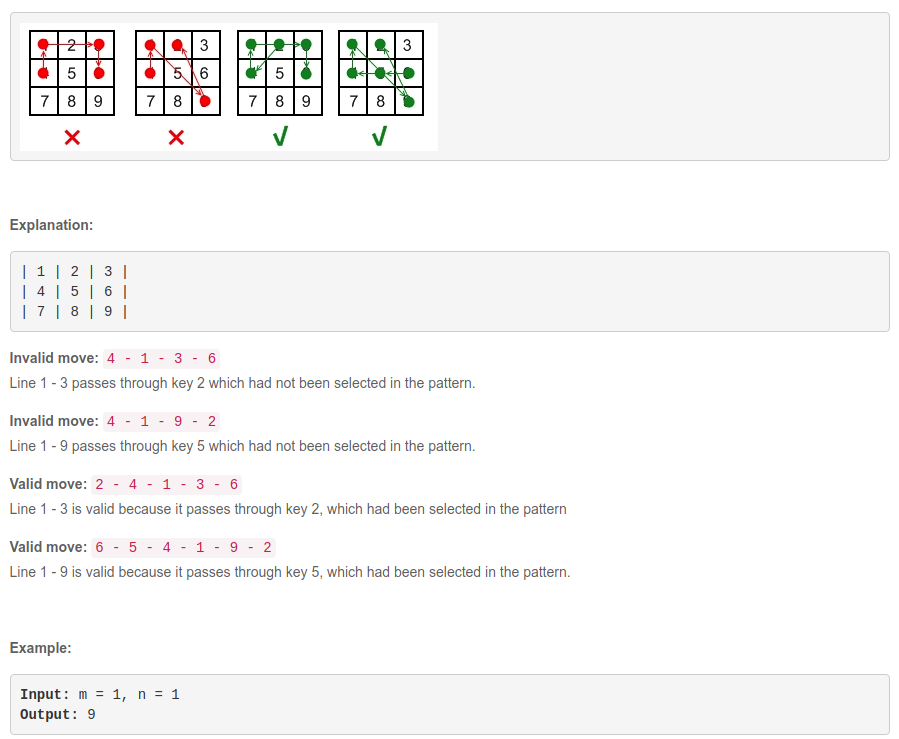
\includegraphics[width=300pt]{android-unlock-patterns.png}\\
\figcaption{Android Unlock Patterns}\label{fig:android-unlock-patterns}
\end{center}

\subsubsection{遞歸 - DFS - vector 版}
\begin{Code}
// 時間複雜度O(N!),空間複雜度O(N)
class Solution {
public:
    int numberOfPatterns(int m, int n) {
        int result = 0;

        // 使用了vector,此方法最慢,對比使用 integer
        vector<bool> used(9, false);
        for (int len = m; len <= n; len++)
            result += DFS(-1, len, used);

        return result;
    }
private:
    // index: 為是次選中的下標 last: 為上次選中的下標
    // IsValid: 是在檢驗,由 last index 走到 index 是否合法
    bool IsValid(int index, int last, const vector<bool>& used)
    {
        // 若果此下標已被使用
        if (used[index]) return false;
        // 若果此下標是第一次被選用
        if (last == -1) return true;
        // 若果是鄰近的移動,或日字移動法
        if ((index + last) % 2 == 1) return true;
        // 若果是大斜角走,要先檢查居中下標
        int mid = (index + last) / 2;
        if (mid == 4) return used[mid];
        // 處理鄰近斜角移動
        if ((index % 3 != last % 3) && (index / 3 != last / 3))
            return true;
        // 剩下的移動選擇都不是相鄰的
        return used[mid];
    }
    int DFS(int last, int len, vector<bool>& used)
    {
        if (len == 0)
            return 1;
        int sum = 0;
        for (int i = 0; i < 9; i++)
        {
            if (IsValid(i, last, used))
            {
                used[i] = true;
                sum += DFS(i, len - 1, used);
                used[i] = false;
            }
        }
        return sum;
    }
};
\end{Code}

\subsubsection{遞歸 - DFS - int 版}
\begin{Code}
// 時間複雜度O(N!),空間複雜度O(N)
// 快很多的版本,因為用了 int 來代替 vector,用來記錄使用情況
class Solution {
public:
    int numberOfPatterns(int m, int n) {
        // 使用 int 來記錄已使用的情況
        return count(m, n, 0, 1, 1);
    }
private:
    int count(int m, int n, int used, int i2, int j2) {
        int number = m <= 0;
        if (!n) return 1;
        for (int i=0; i<3; i++) {
            for (int j=0; j<3; j++) {
                // 求得下一個下標,和標示使用
                int I = i2 + i, J = j2 + j, used2 = used | (1 << (i*3 + j));
                // 當 used2 == used,代表重覆使用下標
                // 所以只有當 used2 變大了才會繼續
                // I % 2 和 J % 2 的檢查包括了所有小斜步和日字步
                // 那後的 (I*3 + J)/2 會檢查大斜步的居中下標和餘下的所有步法
                if (used2 > used && (I % 2 || J % 2 || used2 & (1 << (I/2*3 + J/2))))
                    number += count(m-1, n-1, used2, i, j);
            }
        }
        return number;
    }
};
\end{Code}

\subsubsection{遞歸 - DFS - int 版}
\begin{Code}
// 時間複雜度O(N!),空間複雜度O(N)
// 快很多的版本,因為用了 int 來代替 vector,用來記錄使用情況
class Solution {
public:
    int numberOfPatterns(int m, int n) {
        int result = 0;

        int used = 0;
        for (int len = m; len <= n; len++)
            result += DFS(-1, len, used);

        return result;
    }
private:
    // index: 為是次選中的下標 last: 為上次選中的下標
    // IsValid: 是在檢驗,由 last index 走到 index 是否合法
    bool IsValid(int index, int last, const int& used)
    {
        // 若果此下標已被使用
        if (used & 1 << index) return false;
        // 若果此下標是第一次被選用
        if (last == -1) return true;
        // 若果是鄰近的移動,或日字移動法
        if ((index + last) % 2 == 1) return true;
        // 若果是大斜角走,要先檢查居中下標
        int mid = (index + last) / 2;
        if (mid == 4) return used & 1 << mid;
        // 處理鄰近斜角移動
        if ((index % 3 != last % 3) && (index / 3 != last / 3))
            return true;
        // 剩下的移動選擇都不是相鄰的
        return used & 1 << mid;
    }
    int DFS(int last, int len, int& used)
    {
        if (len == 0)
            return 1;
        int sum = 0;
        for (int i = 0; i < 9; i++)
        {
            if (IsValid(i, last, used))
            {
                used |= 1 << i;
                sum += DFS(i, len - 1, used);
                used &= ~(1 << i);
            }
        }
        return sum;
    }
};
\end{Code}

\section{Fenwick Tree or Binary Indexed Tree} %%%%%%%%%%%%%%%%%%%%%%%%%%%%%%
\label{sec:fenwick-tree-or-binary-indexed-tree}


\subsubsection{描述}
We may use this tree to calculate the sum of the prefix of a given array. Mean while we can update the value of the array and the tree in logN time.

\subsubsection{Code}
\begin{Code}
// 時間複雜度O(NLogN),空間複雜度O(N)
// Learn from https://www.youtube.com/watch?v=CWDQJGaN1gY
class FenwickTree
{
public:
    FenwickTree() {}
    ~FenwickTree() {}

    vector<int> CreateTree(const vector<int>& input)
    {
        vector<int> binaryIndexedTree(input.size()+1);

        for (size_t i = 1; i <= input.size(); i++)
        {
            UpdateBinaryIndexedTree(binaryIndexedTree, input[i-1], i);
        }
        return binaryIndexedTree;
    }
    int GetSum(const vector<int>& binaryIndexedTree, int index)
    {
        index++;
        int sum = 0;
        while (index > 0)
        {
            sum += binaryIndexedTree[index];
            index = GetParent(index);
        }
        return sum;
    }
private:
    void UpdateBinaryIndexedTree(vector<int>& binaryIndexedTree, int val, int index)
    {
        while (index < binaryIndexedTree.size())
        {
            binaryIndexedTree[index] += val;
            index = GetNext(index);
        }
    }
    /**
     * To get parent
     * 1) 2's complement to get minus of index
     * 2) AND this with index
     * 3) Subtract that from index
     */
    int GetParent(int index)
    {
        return index - (index & -index);
    }
    /**
     * To get next
     * 1) 2's complement of get minus of index
     * 2) AND this with index
     * 3) Add it to index
     */
    int GetNext(int index)
    {
        return index + (index & -index);
    }
};
int main(int argc, char *argv[])
{
    vector<int> input{1,2,3,4,5,6,7};
    FenwickTree ft;
    vector<int> binaryIndexedTree = ft.CreateTree(input);
    assert(1 == ft.GetSum(binaryIndexedTree, 0));
    assert(3 == ft.GetSum(binaryIndexedTree, 1));
    assert(6 == ft.GetSum(binaryIndexedTree, 2));
    assert(10 == ft.GetSum(binaryIndexedTree, 3));
    assert(15 == ft.GetSum(binaryIndexedTree, 4));
    assert(21 == ft.GetSum(binaryIndexedTree, 5));
    assert(28 == ft.GetSum(binaryIndexedTree, 6));

    return 0;
}
\end{Code}

\section{Count of Smaller Numbers After Self} %%%%%%%%%%%%%%%%%%%%%%%%%%%%%%
\label{sec:count-of-smaller-numbers-after-self}

\subsubsection{描述}
You are given an integer array nums and you have to return a new counts array. The counts array has the property where counts[i] is the number of smaller elements to the right of nums[i].

Example:
\begin{Code}
Input: [5,2,6,1]
Output: [2,1,1,0] 
Explanation:
To the right of 5 there are 2 smaller elements (2 and 1).
To the right of 2 there is only 1 smaller element (1).
To the right of 6 there is 1 smaller element (1).
To the right of 1 there is 0 smaller element.
\end{Code}

Note:
Please read more about FenwickTree from example FenwickTree.

\subsubsection{Code}
\begin{Code}
// 時間複雜度O(NLogN),空間複雜度O(N)
// The idea of this solution is similar to the monotonic stack
class Solution {
public:
    vector<int> countSmaller(vector<int>& nums)
    {
        // Relative indexing.
        // This is the key to achieve true O(n(log(n))).
        set<int> unique_elements;
        for (const int& i : nums) unique_elements.insert(i);

        // 由細至大配上 id
        unordered_map<int,int> index;
        int id = 0;
        for (const auto& e : unique_elements) index[e] = id++;

        // Fenwick Tree
        vector<int> ft(id+1);

        vector<int> result;
        // 由尾至頭歷遍
        for (int i = nums.size()-1; i >= 0; --i)
        {
            // 記低出現過的下標
            ftIncrement(ft, index[nums[i]]);
            // 數一數較細的下標出現過的次數
            result.push_back(ftPrefixSum(ft, index[nums[i]]));
        }
        reverse(result.begin(),result.end());
        return result;
    }
private:
    // Insert into Fenwick tree
    // O(log(n))
    void ftIncrement(vector<int> &ft, int index)
    {
        // 0 index -> 1 index
        ++index;
        while (index < ft.size())
        {
            ft[index] += 1;
            index += (index&-index);
        }
    }
    // Get sum from [0,index) in a Fenwick tree.
    // O(log(n))
    int ftPrefixSum(vector<int> &ft, int index)
    {
        // 0 index -> 1 index but excluding index
        int sum = 0;
        while (index > 0)
        {
            sum += ft[index];
            index -= (index&-index);
        }
        return sum;
    }
};
\end{Code}

\section{Coin Change} %%%%%%%%%%%%%%%%%%%%%%%%%%%%%%
\label{sec:coin-change}

\subsubsection{描述}
You are given coins of different denominations and a total amount of money amount. Write a function to compute the fewest number of coins that you need to make up that amount. If that amount of money cannot be made up by any combination of the coins, return -1.

Example 1:
\begin{Code}
Input: coins = [1, 2, 5], amount = 11
Output: 3 
Explanation: 11 = 5 + 5 + 1
\end{Code}

Example 2:
\begin{Code}
Input: coins = [2], amount = 3
Output: -1
\end{Code}

Note:
You may assume that you have an infinite number of each kind of coin.

\subsubsection{DP}
設狀態為$f(i)$,表示\fn{i}最少的 coins 數目
$$
f(i) = min(f(i-coins[j]) + 1) \&\& coins[j] < i
$$

\begin{Code}
// 時間複雜度O(n*k),空間複雜度O(n)
class Solution {
public:
    int coinChange(vector<int>& coins, int amount) {
        if (coins.size() == 0) return -1;
        sort(coins.begin(), coins.end());

        vector<int> f(amount+1, INT_MAX);
        f[0] = 0;

        for (int i = coins[0]; i < f.size(); i++)
        {
            for (int j = 0; j < coins.size(); j++)
            {
                if (coins[j] > i) break;
                if (f[i-coins[j]] == INT_MAX) continue;
                f[i] = min(f[i], f[i-coins[j]] + 1);
            }
        }

        return f[amount] == INT_MAX ?  -1 : f[amount];
    }
};
\end{Code}

\subsubsection{DFS}
\begin{Code}
// 時間複雜度O(n*k),空間複雜度O(n)
class Solution {
public:
    int coinChange(vector<int>& coins, int amount) {
        if (coins.size() == 0) return -1;
        sort(coins.begin(), coins.end());

        vector<int> counts(amount+1, 0);
        counts[0] = 0;
        DFS(coins, amount, counts);

        return counts[amount] == INT_MAX ? -1 : counts[amount];
    }
private:
    int DFS(vector<int>& coins, int amount, vector<int>& counts)
    {
        if (amount < 0) return -1;
        if (amount == 0) return 0;
        if (counts[amount] != 0) return counts[amount];
        else
        {
            int minCount = INT_MAX;
            for (int i = coins.size() - 1; i >= 0; i--)
            {
                if (coins[i] > amount) continue;
                int ret = DFS(coins, amount-coins[i], counts);
                if (ret >= 0 && ret < minCount)
                    minCount = 1 + ret;
            }
            return counts[amount] = minCount == INT_MAX ? -1 : minCount;
        }
    }
};
\end{Code}

\section{Min Stack} %%%%%%%%%%%%%%%%%%%%%%%%%%%%%%
\label{sec:min-stack}

\subsubsection{描述}
Design a stack that supports push, pop, top, and retrieving the minimum element in constant time.

\begindot
\item push(x) -- Push element x onto stack.
\item pop() -- Removes the element on top of the stack.
\item top() -- Get the top element.
\item getMin() -- Retrieve the minimum element in the stack.
\myenddot

Example 1:
\begin{Code}
Input
["MinStack","push","push","push","getMin","pop","top","getMin"]
[[],[-2],[0],[-3],[],[],[],[]]

Output
[null,null,null,null,-3,null,0,-2]

Explanation
MinStack minStack = new MinStack();
minStack.push(-2);
minStack.push(0);
minStack.push(-3);
minStack.getMin(); // return -3
minStack.pop();
minStack.top();    // return 0
minStack.getMin(); // return -2
\end{Code}


Note:
You may assume that you have an infinite number of each kind of coin.

\subsubsection{Stack and Min Stack}
\begin{Code}
// 時間複雜度O(1),空間複雜度O(n)
class MinStack {
public:
    MinStack(){

    }
    void push(int x)
    {
        if(s1.empty())
        {
            s1.push(x);
            minStack.push(x);
        }
        else
        {
            if(x < minStack.top())
            {
                s1.push(x);
                minStack.push(x);
            }
            else
            {
                s1.push(x);
                minStack.push(minStack.top());
            }
        }
    }
    void pop()
    {
        s1.pop();
        minStack.pop();
    }
    int top()
    {
        return s1.top();
    }
    int getMin()
    {
        return minStack.top();
    }
private:
    stack<int> s1; // 一個正常 stack
    stack<int> minStack; // 一個 min stack
};
\end{Code}

\subsubsection{Stack and Pair}
\begin{Code}
// 時間複雜度O(1),空間複雜度O(n)
class MinStack {
public:
    /** initialize your data structure here. */
    MinStack() {

    }

    void push(int x) {
        if (m_cache.empty())
            m_cache.emplace(x, x);
        else
            m_cache.emplace(x, min(m_cache.top().second, x));
    }

    void pop() {
        m_cache.pop();
    }

    int top() {
        return m_cache.top().first;
    }

    int getMin() {
        return m_cache.top().second;
    }
private:
    stack<pair<int,int>> m_cache;
};
\end{Code}

\section{Guess the Word} %%%%%%%%%%%%%%%%%%%%%%%%%%%%%%
\label{sec:guess-the-word}

\subsubsection{描述}
This problem is an interactive problem new to the LeetCode platform.

We are given a word list of unique words, each word is 6 letters long, and one word in this list is chosen as secret.

You may call master.guess(word) to guess a word.  The guessed word should have type string and must be from the original list with 6 lowercase letters.

This function returns an integer type, representing the number of exact matches (value and position) of your guess to the secret word.  Also, if your guess is not in the given wordlist, it will return -1 instead.

For each test case, you have 10 guesses to guess the word. At the end of any number of calls, if you have made 10 or less calls to master.guess and at least one of these guesses was the secret, you pass the testcase.

Besides the example test case below, there will be 5 additional test cases, each with 100 words in the word list.  The letters of each word in those testcases were chosen independently at random from 'a' to 'z', such that every word in the given word lists is unique.

Example 1:
\begin{Code}
Input: secret = "acckzz", wordlist = ["acckzz","ccbazz","eiowzz","abcczz"]

Explanation:

master.guess("aaaaaa") returns -1, because "aaaaaa" is not in wordlist.
master.guess("acckzz") returns 6, because "acckzz" is secret and has all 6 matches.
master.guess("ccbazz") returns 3, because "ccbazz" has 3 matches.
master.guess("eiowzz") returns 2, because "eiowzz" has 2 matches.
master.guess("abcczz") returns 4, because "abcczz" has 4 matches.

We made 5 calls to master.guess and one of them was the secret, so we pass the test case.
\end{Code}


Note:
Any solutions that attempt to circumvent the judge will result in disqualification.

\subsubsection{Minimax Strategy}
\begin{Code}
// 時間複雜度O(N^2),空間複雜度O(N^2)
// 使用了 minimax algorithm 來最大化地減少下一個需要嘗試的搜尋範圍
class Solution {
public:
    void findSecretWord(vector<string>& wordlist, Master& master) {
        int N = wordlist.size();
        m_H.resize(N, vector<int>(N));
        for (int i = 0; i < N; i++)
        {
            for (int j = i; j < N; j++)
            {
                int match = 0;
                for (int k = 0; k < 6; k++)
                {
                    if (wordlist[i][k] == wordlist[j][k])
                        match++;
                }
                m_H[i][j] = m_H[j][i] = match;
            }
        }

        vector<int> possible;
        vector<bool> path(N, false);
        for (int i = 0; i < N; i++) possible.push_back(i);

        while (!possible.empty())
        {
            int guess = solve(possible, path);
            int matches = master.guess(wordlist[guess]);
            if (matches == wordlist[0].length()) return; // 找到答案

            // 找不到答案,便需要找出下一個搜尋範圍
            vector<int> possible2;
            for (const int& j : possible)
                if (m_H[guess][j] == matches) possible2.push_back(j);
            possible = possible2;
            path[guess] = true;
        }
    }
private:
    vector<vector<int>> m_H;

    int solve(const vector<int>& possible, const vector<bool>& path)
    {
        if (possible.size() <= 2) return possible.front();
        int ansgrpSize = possible.size();
        int ansguess = -1;

        for (int guess = 0; guess < m_H.size(); guess++)
        {
            if (!path[guess])
            {
                vector<vector<int>> groups(7, vector<int>());
                for (const int& j : possible)
                {
                    if (j != guess)
                        groups[m_H[guess][j]].push_back(j);
                }

                int maxGroupSize = 0;
                for (int i = 0; i < 7; i++)
                {
                    if (groups[i].size() > maxGroupSize)
                        maxGroupSize = groups[i].size();
                }

                if (maxGroupSize < ansgrpSize)
                {
                    ansgrpSize = maxGroupSize;
                    ansguess = guess;
                }
            }
        }

        return ansguess;
    }
};
\end{Code}

\subsubsection{Random Pick}
\begin{Code}
// 時間複雜度O(N^2),空間複雜度O(N^2)
class Solution {
public:
    void findSecretWord(vector<string>& wordlist, Master& master) {

        string target = wordlist[rand() % wordlist.size()];
        int count = 10;
        while(count--) {
            int numMatch = master.guess(target);

            shrinkList(wordlist, target, numMatch);

            target = wordlist[rand() % wordlist.size()];
        }
    }

private:
    void shrinkList(vector<string> & wordlist, const string & target, int numMatch) {
        vector<string> newList;
        for (auto & w : wordlist) {
            if (computeComm(w, target) == numMatch) {
                newList.push_back(w);
            }
        }
        wordlist = newList;
    }

    int computeComm(const string & s1, const string & s2) {
        int comm = 0;
        for (int i = 0; i < 6; ++i) {
            if (s1[i] == s2[i]) comm++;
        }
        return comm;
    }

};
\end{Code}
